
It the previous chapter the proposed load balancer is verified to be portable, redundant and scalable in 1Gbps network.
It is important to investigate its validity also in 10Gbps network.
In this chapter the performance level of the proposed load balancer is evaluated.
The author carries out throughput measurements of ipvs, ipvs-tun, and iptables DNAT in 10Gbps environment.
The author clarifies the reasons for performance limitations and discusses improvement.
The author also proposes a novel software load balancer using eXpress Data Plane(XDP) technology and presents preliminary experimental results.

\section{Throughput measurement in 10G network}

In order to evaluate the performance levels of the proposed load balancer in a 10Gbps network environment, the author carried out throughput measurements.
Table~\ref{tab:hw_sw_spec_10g} summarizes the hardware and software specification used in the experiment.
Bare metal servers with Intel X550 network card was used.
The X550 NIC has a maximum of 64 rx-queues, and at the boot time, 16 of them are activated by the driver since there are 16 logical CPUs.
The setting \enquote{(RSS, RPS)=(on, off)} is used because interrupts from each of 16 rx-queues can be assigned to separate logical cores.
As a result, packet processing is distributed to all of the cores, which results in the best performance in most of the cases.

{
\setlength{\tabcolsep}{1em}
\renewcommand{\arraystretch}{1.2}

\begin{table}[h]
  \centering
  \begin{tabular}{ll}
    \hline 
    \multicolumn{2}{l}{[Hardware Specification]}   \\
    & CPU: Xeon E5-2450 2.10GHz x 8 (with Hyper Threading) \\
    & Memory: 32GB \\
    & NIC: Intel X550 with 64 rx-queues (16 activated), 10 Gbps \\
    & (Node x 6, Load Balancer x 1, Client x 1)) \\
    & \\
    \multicolumn{2}{l}{[Node Software]}  \\
    & OS: Debian 9.5, linux-4.16.8 \\
    & Kubernetes v1.5.2 \\
    & flannel v0.7.0 \\
    & etcd version: 3.0.15 \\
    & \\
    \multicolumn{2}{l}{[Container Software]}   \\
    & Keepalived: v1.3.2 (12/03,2016) \\
    & nginx : 1.15.4(web server) \\
  \hline 
  \end{tabular}
  \par\bigskip
  \centering
  \begin{minipage}{0.9\columnwidth}
    \caption[Hardware and software specifications for 10Gbps experiment]{
      Hardware and software specifications for 10Gbps experiment.
      There are 16 rx-queues activated for the NIC, to match the number of logical CPUs.
    }
    \label{tab:hw_sw_spec_10g}
  \end{minipage}
\end{table}
}

\begin{figure}[h]
  \begin{subfigure}[t]{\columnwidth}
    \centering
    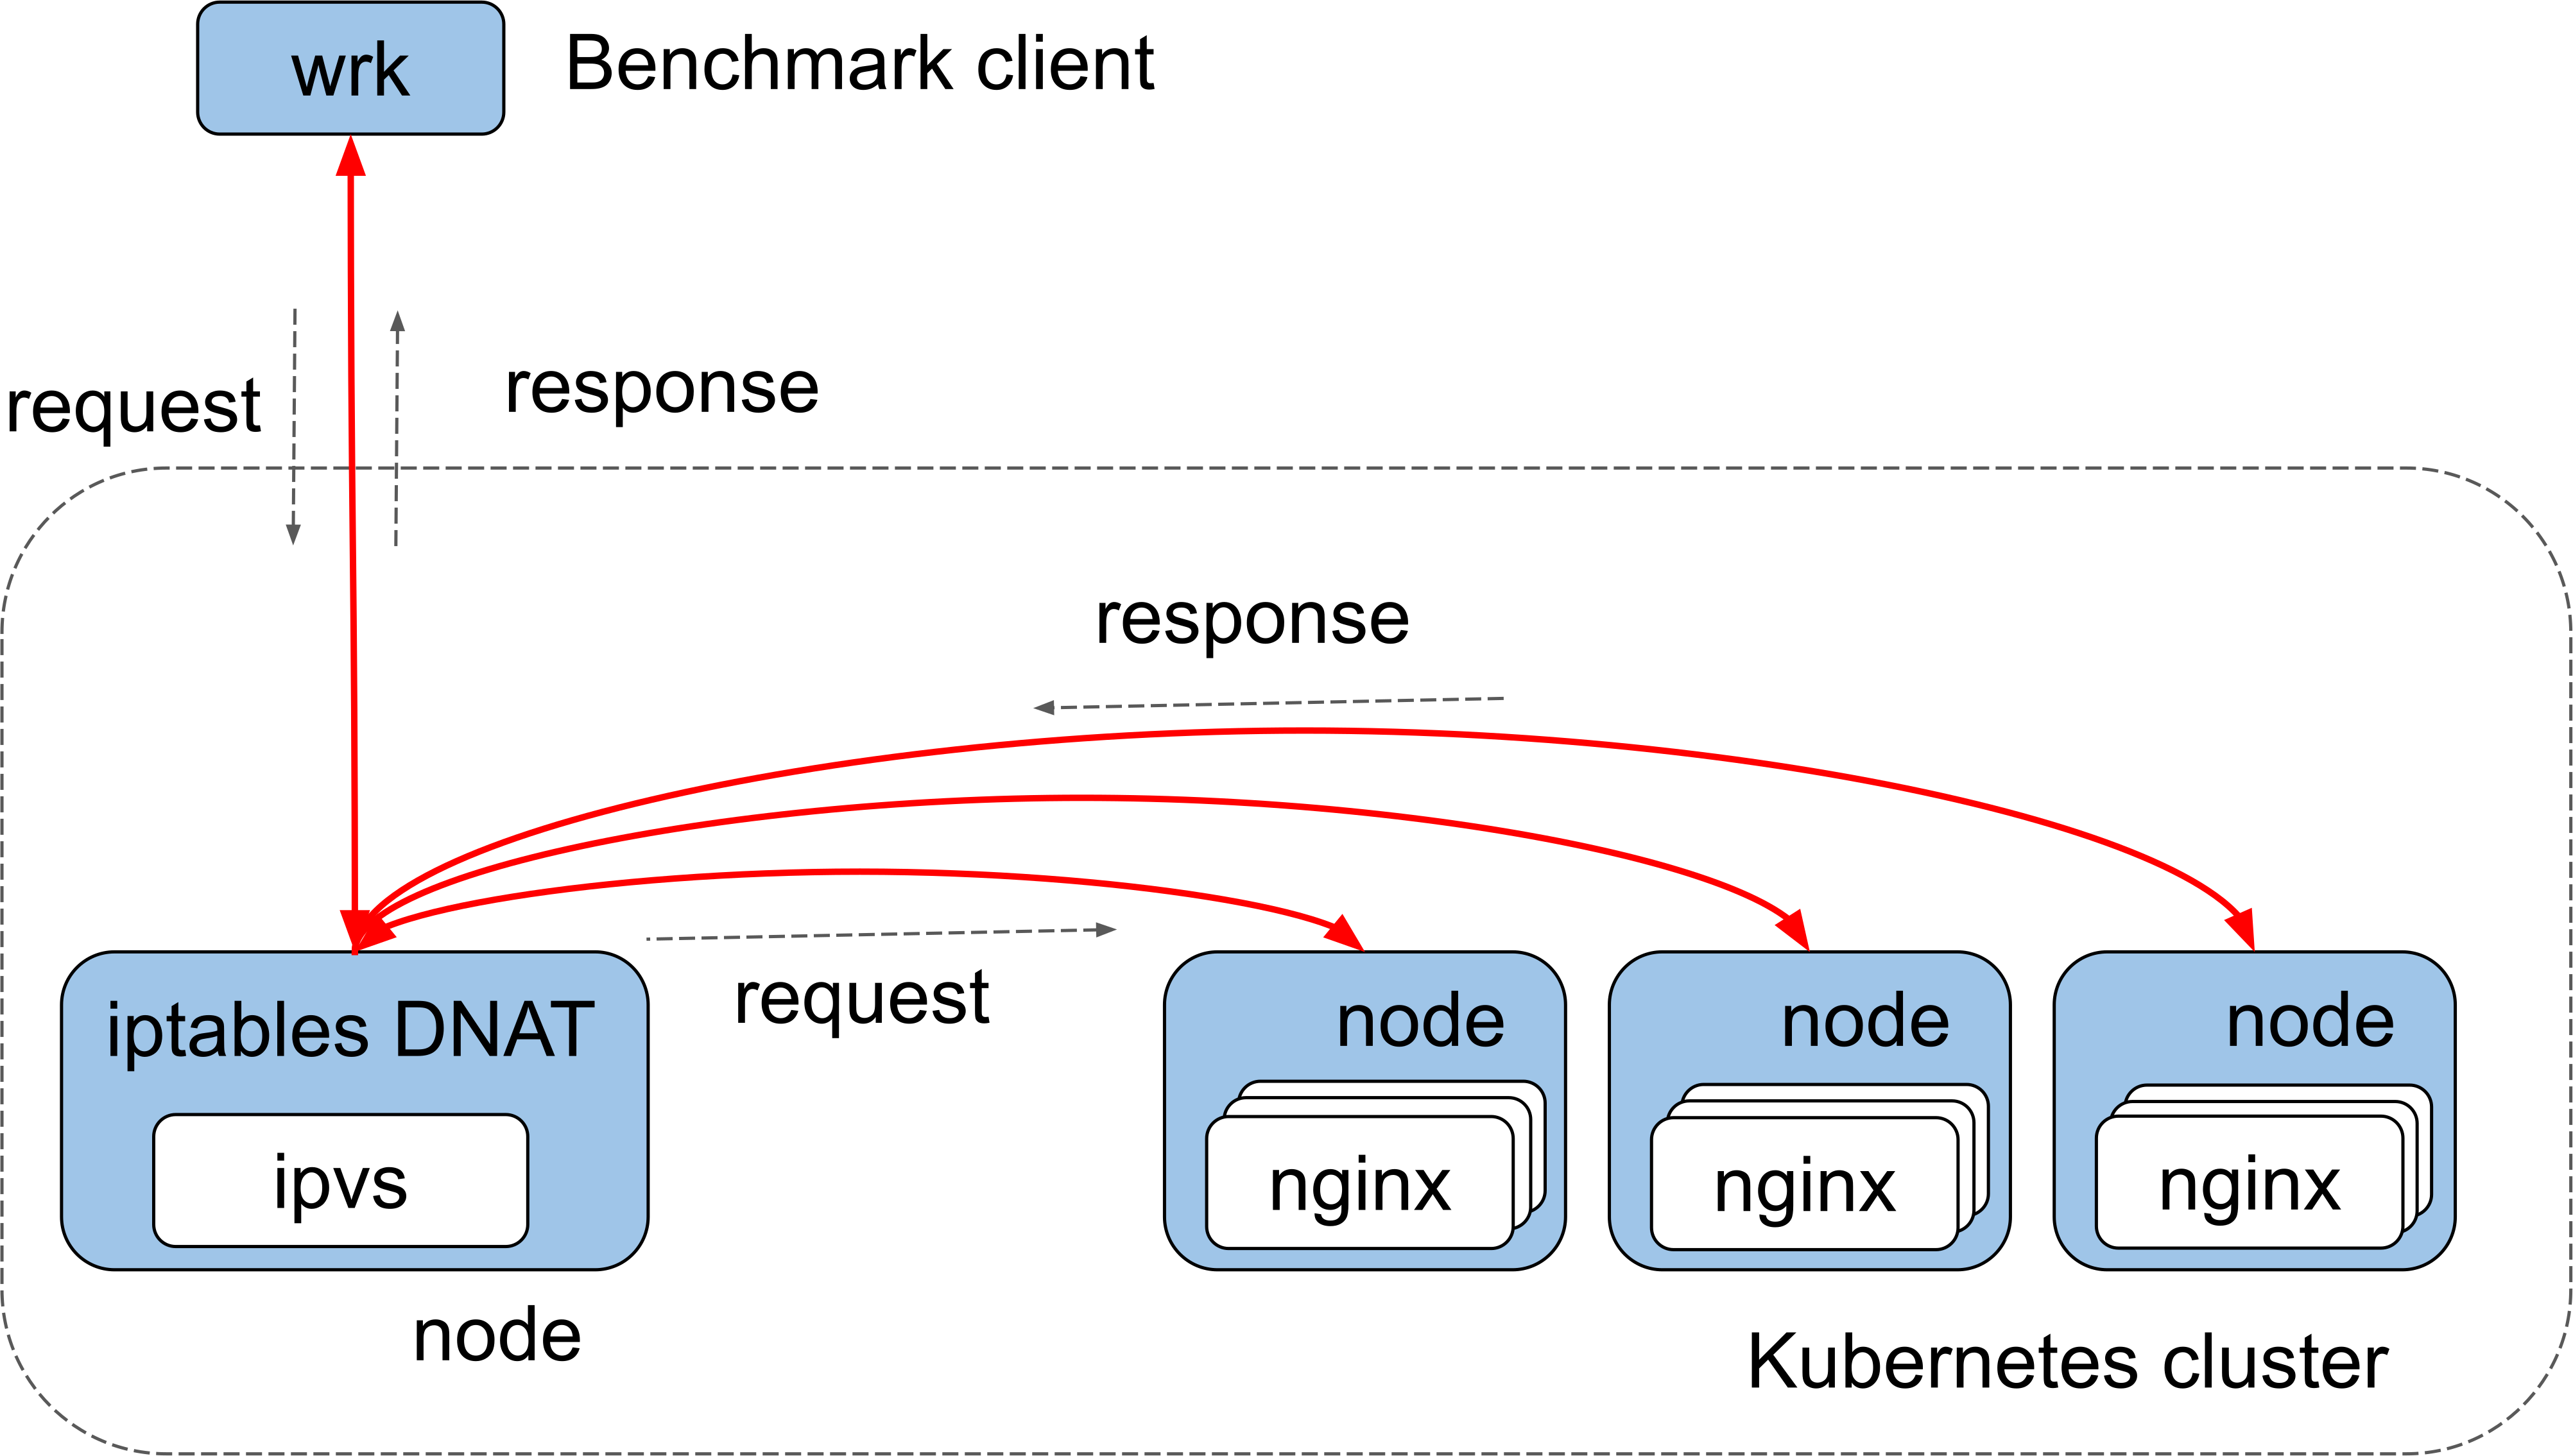
\includegraphics[width=0.8\columnwidth]{Figs/benchmark-schem-10g-nat}
    \par\bigskip
    \centering
    \begin{minipage}{0.9\columnwidth}
      \caption{}
      \label{fig:benchmark-schem-10g-nat}
    \end{minipage}
  \end{subfigure}

  \begin{subfigure}[t]{\columnwidth}
    \centering
    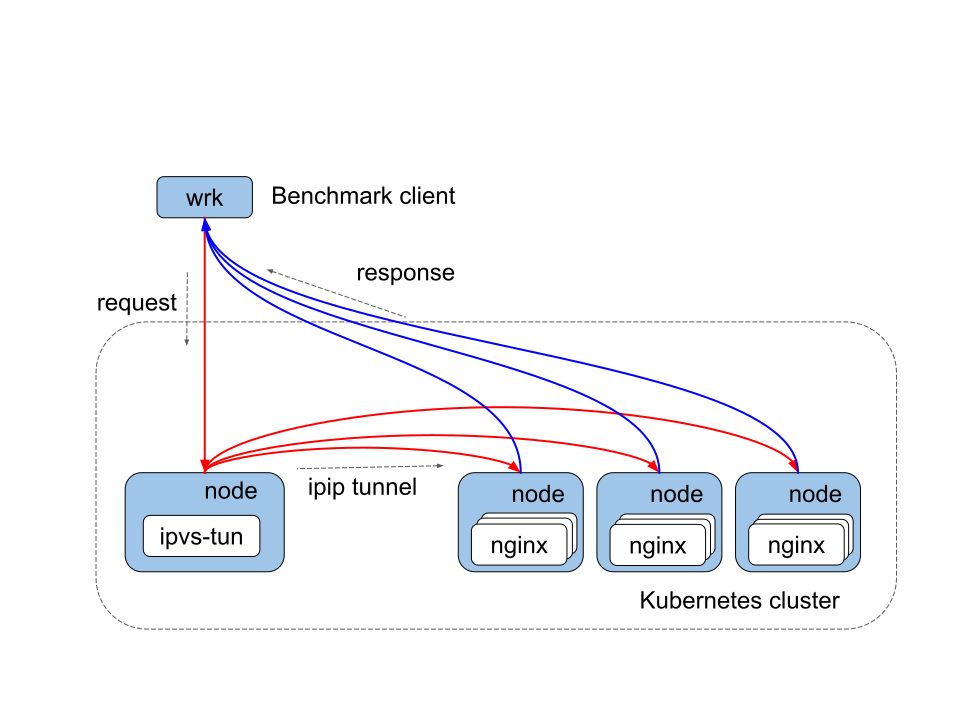
\includegraphics[width=0.8\columnwidth]{Figs/benchmark-schem-10g-dsr}
    \par\bigskip
    \centering
    \begin{minipage}{0.9\columnwidth}
      \caption{}
      \label{fig:benchmark-schem-10g-dsr}
    \end{minipage}
  \end{subfigure}

  \par\bigskip
  \centering
  \begin{minipage}{0.9\columnwidth}
    \caption[Benchmark setups in 10 Gbps experiment]{
      Benchmark setups in 10 Gbps experiment.
      (a) The setup used in throughput measurements of ipvs and iptables DNAT.
      The request and response packets both go through the load balancer node.
      There is a bottleneck at the NIC of the load balancer node.
      (b) The setup used in throughput measurements of ipvs-tun.
      The response packets for ipvs-tun, return directly to the benchmark client.
      The bottleneck is at the NIC of the benchmark client.
    }
    \label{fig:benchmark-schem-10g}
  \end{minipage}
\end{figure}

Figure~\ref{fig:benchmark-schem-10g} show experimental setups for the throughput measurements.
Multiple nginx {\em pods} are deployed on multiple nodes as web servers in the Kubernetes cluster.
In each nginx {\em pod}, single nginx web server program that returns the IP address of the {\em pod} itself is running.
The author then launched ipvs and ipvs-tun pod as load balancers on one of the nodes, after that, performed the throughput measurement changing the number of the nginx web server pods.
On every Kubernetes node, there are iptables DNAT rules that function as an internal load balancer.
The author also measured throughput for the iptables DNAT as a load balancer.
The throughput is measured by sending out HTTP requests from the wrk towards a load balancer and by counting the number of responses the benchmark client received.
In the case of the ipvs-tun, i.e., the tunneling mode of ipvs, the response packets follow the different route than the case of conventional ipvs and iptables DNAT.
As a result, the better performance level is expected for ipvs-tun since the load balancer node only has to deal with request packets of the traffic.

\FloatBarrier

Figure~\ref{fig:ipvs_l3dsr_10g} shows the throughput results of ipvs, ipvs-tun and iptables DNAT in 10Gbps environment.
The general characteristics of a load balancer, where the throughput increases linearly to a saturation level as the number of nginx container increases, can be seen.
The maximum throughput of each of the load balancers is limited by either packet forwarding efficiency of the software itself or the bandwidth of the network.
The maximum throughput level of the iptables DNAT is close to 780k [req/sec], where the CPU usage of the benchmark client becomes 100\%.
The maximum throughput levels of ipvs and ipvs-tun are less than that of iptables DNAT. 

\begin{figure}[h]
  \centering
  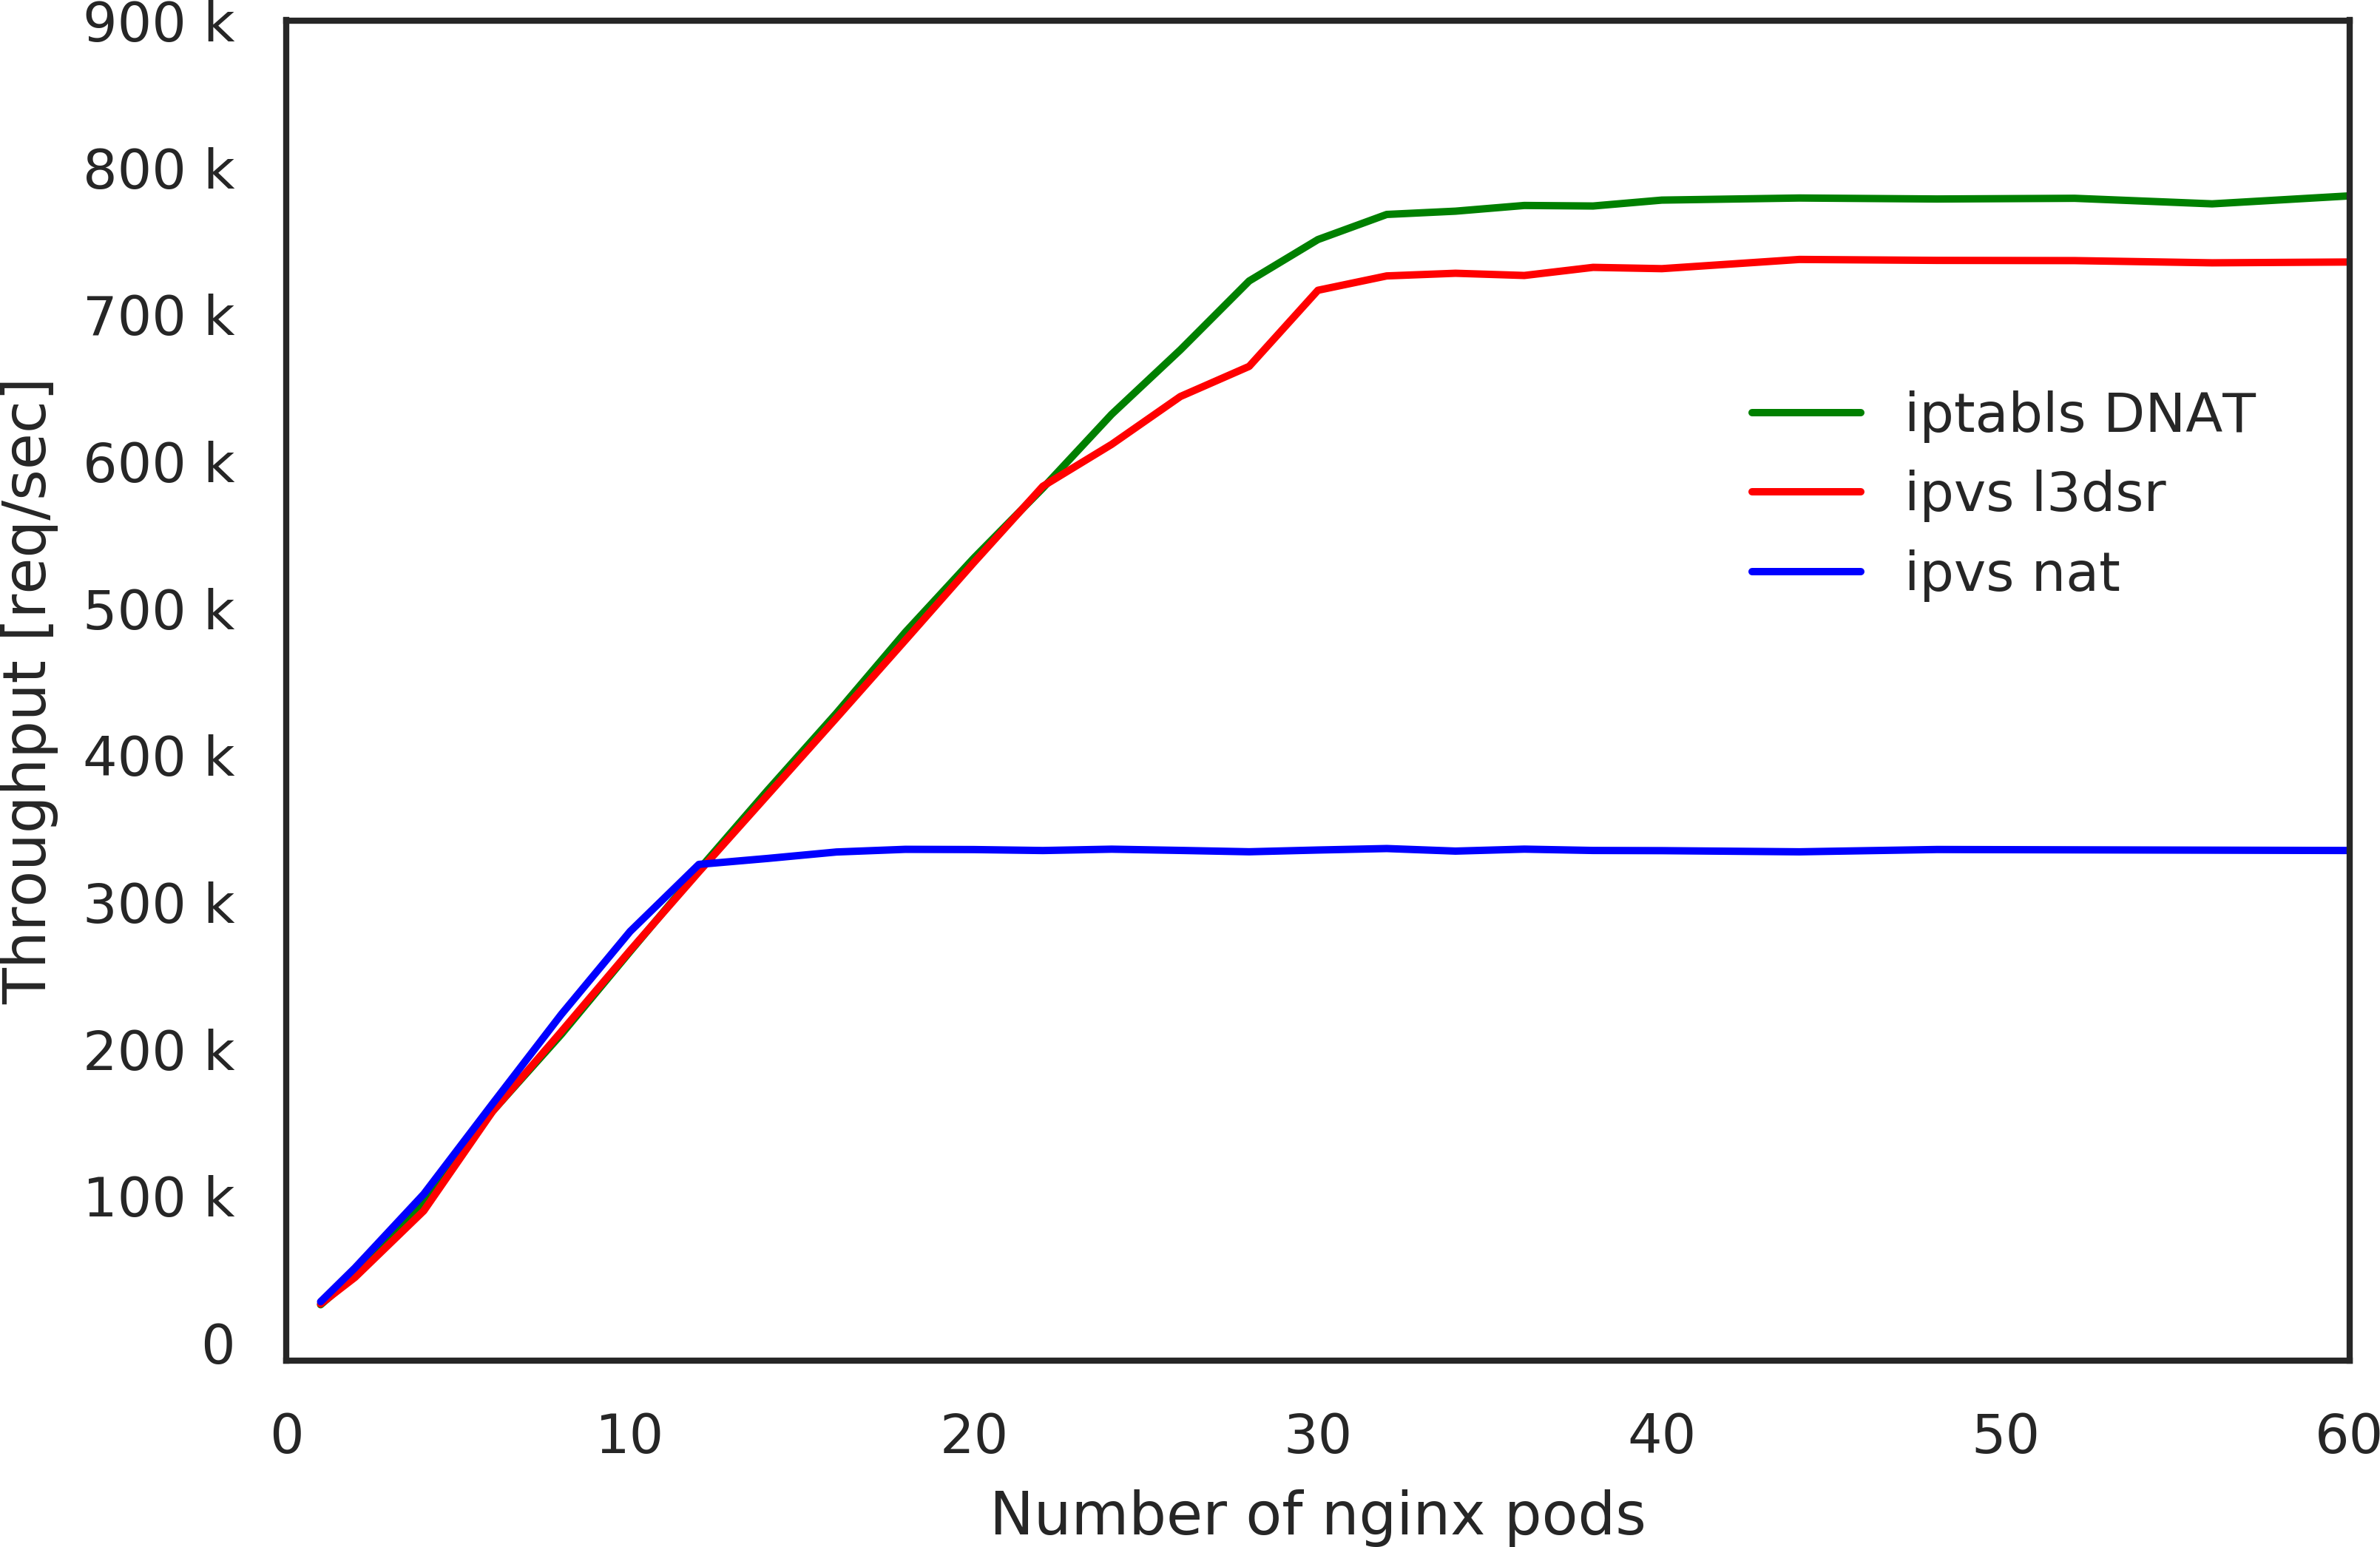
\includegraphics[width=0.8\columnwidth]{Figs/ipvs_l3dsr_10g}
  \par\bigskip
  \centering
  \begin{minipage}{0.9\columnwidth}
    \caption[Throughput of load balancers in 10 Gbps]{
      Throughput of load balancers in 10 Gbps.
      The iptables DNAT rules exist in the node net namespace.
      The ipvs and ipvs-tun are in containers.
      The throughput of the iptables DNAT rules is the highest.
    }
    \label{fig:ipvs_l3dsr_10g}
  \end{minipage}
\end{figure}

Figure~\ref{fig:ipvs_l3dsr_10g} shows comparison of CPU usage between load balancers.
CPU usages are sampled on the load balancer nodes at the time of the throughput measurement using a program called dstat\cite{wieers2019dstat}.
It is seen that ipvs-tun uses less CPU resource than ipvs because the load balancer node does not have to deal with the response packets.
The iptables DNAT uses even less CPU resource than ipvs and ipvs-tun.
Possible reasons for this can be as follows;
(1) It is possible that the ipvs and ipvs-tun program itself is less efficient than iptables DNAT.
(2) The network setup for the container, i.e., bridge+veth may be causing the overhead.
While iptables DNAT rules exist in node net namespace, proposed ipvs and ipvs-tun exist in container net namespace. 
In order to clarify the reason for the performance difference, the author carried out throughput measurement for ipvs and ipvs-tun in node net namespaces.

\begin{figure}[h]
  \centering
  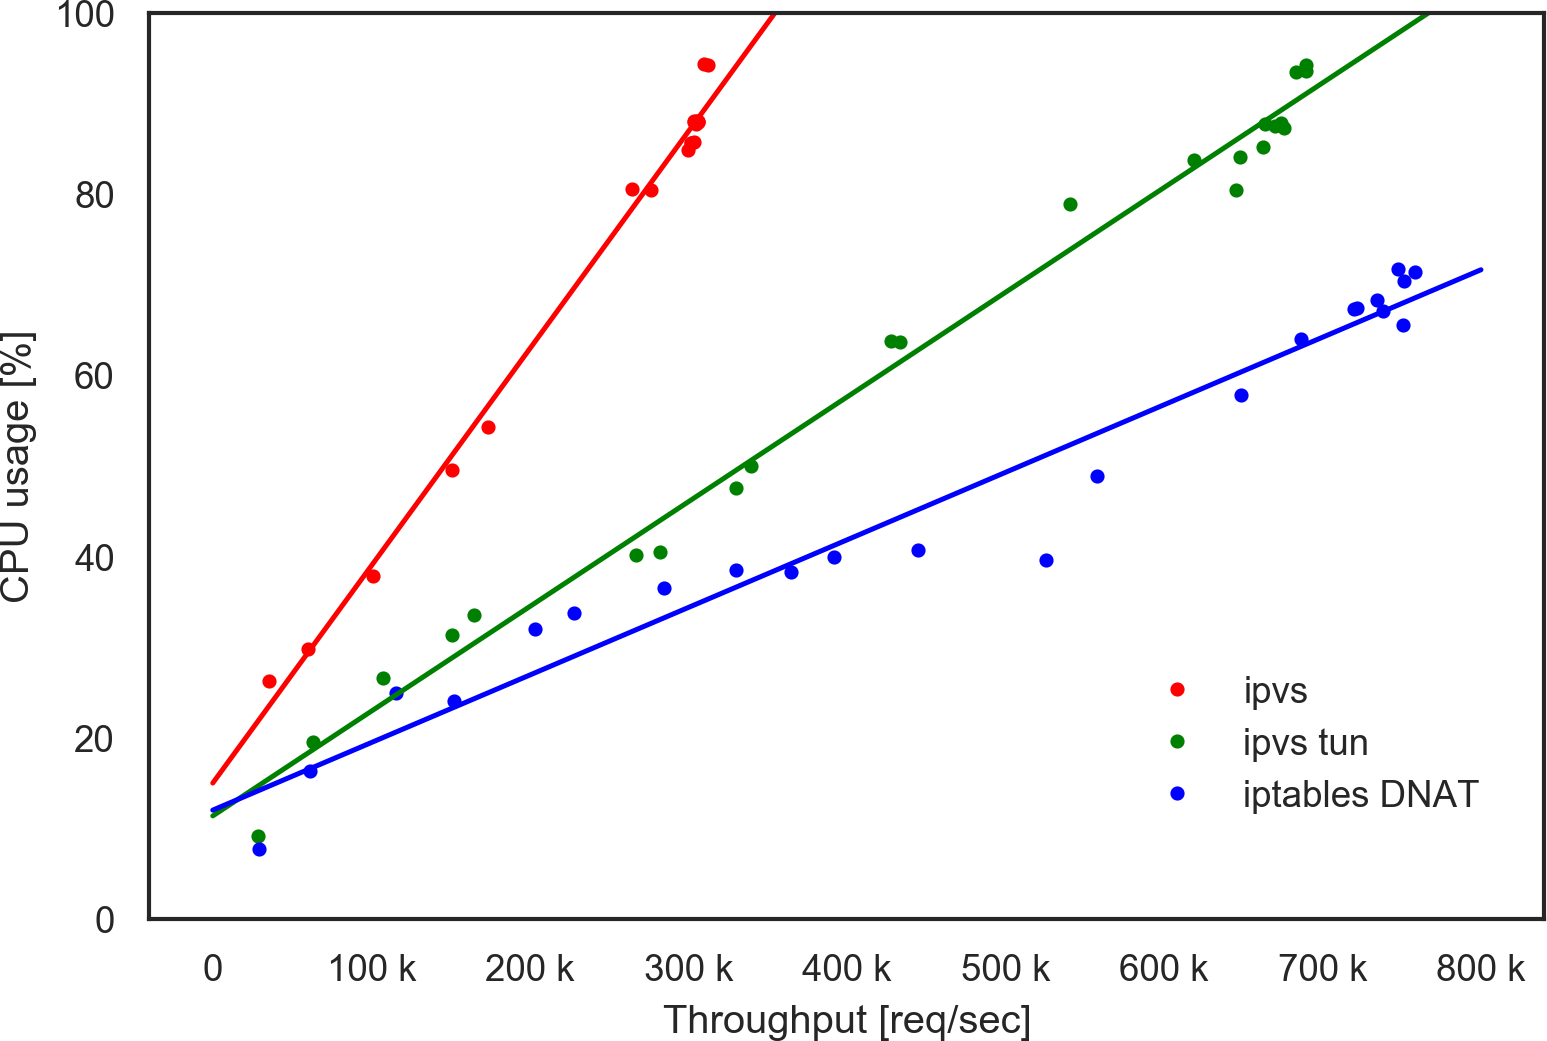
\includegraphics[width=0.8\columnwidth]{Figs/cpu_usage_10g}
  \par\bigskip
  \centering
  \begin{minipage}{0.9\columnwidth}
    \caption[CPU usage of load balancers in containers]{
      CPU usage of load balancers in containers.
      The iptables DNAT rules exist in the node net namespace.
      The ipvs and ipvs-tun are in containers.
      The iptables DNAT consumes the smallest amount of the CPU resource.
    }
    \label{fig:cpu_usage_10g}
  \end{minipage}
\end{figure}

\FloatBarrier

\subsubsection{Performance comparison in node net namespace}

The ipvs and ipvs-tun load balancers were setup on one of the nodes. 
The load balancing rules are created in the node namespaces, and then throughput measurement were carried out.

Figure~\ref{fig:ipvs_node_l3dsr_10g} shows the throughput of ipvs and ipvs-tun in the node net namespace together with the throughput of the iptables DNAT.
The throughputs of the ipvs and ipvs-tun are improved from the previous results.
The throughput of the ipvs-tun is almost identical to that of iptables DNAT.
The CPU usages of the benchmark client at saturated throughput were almost 100\% for both ipvs-tun and iptables DNAT. 
On the other hand, the throughput of ipvs is still less than those of ipvs-tun and iptables DNAT.

\begin{figure}[h]
  \centering
  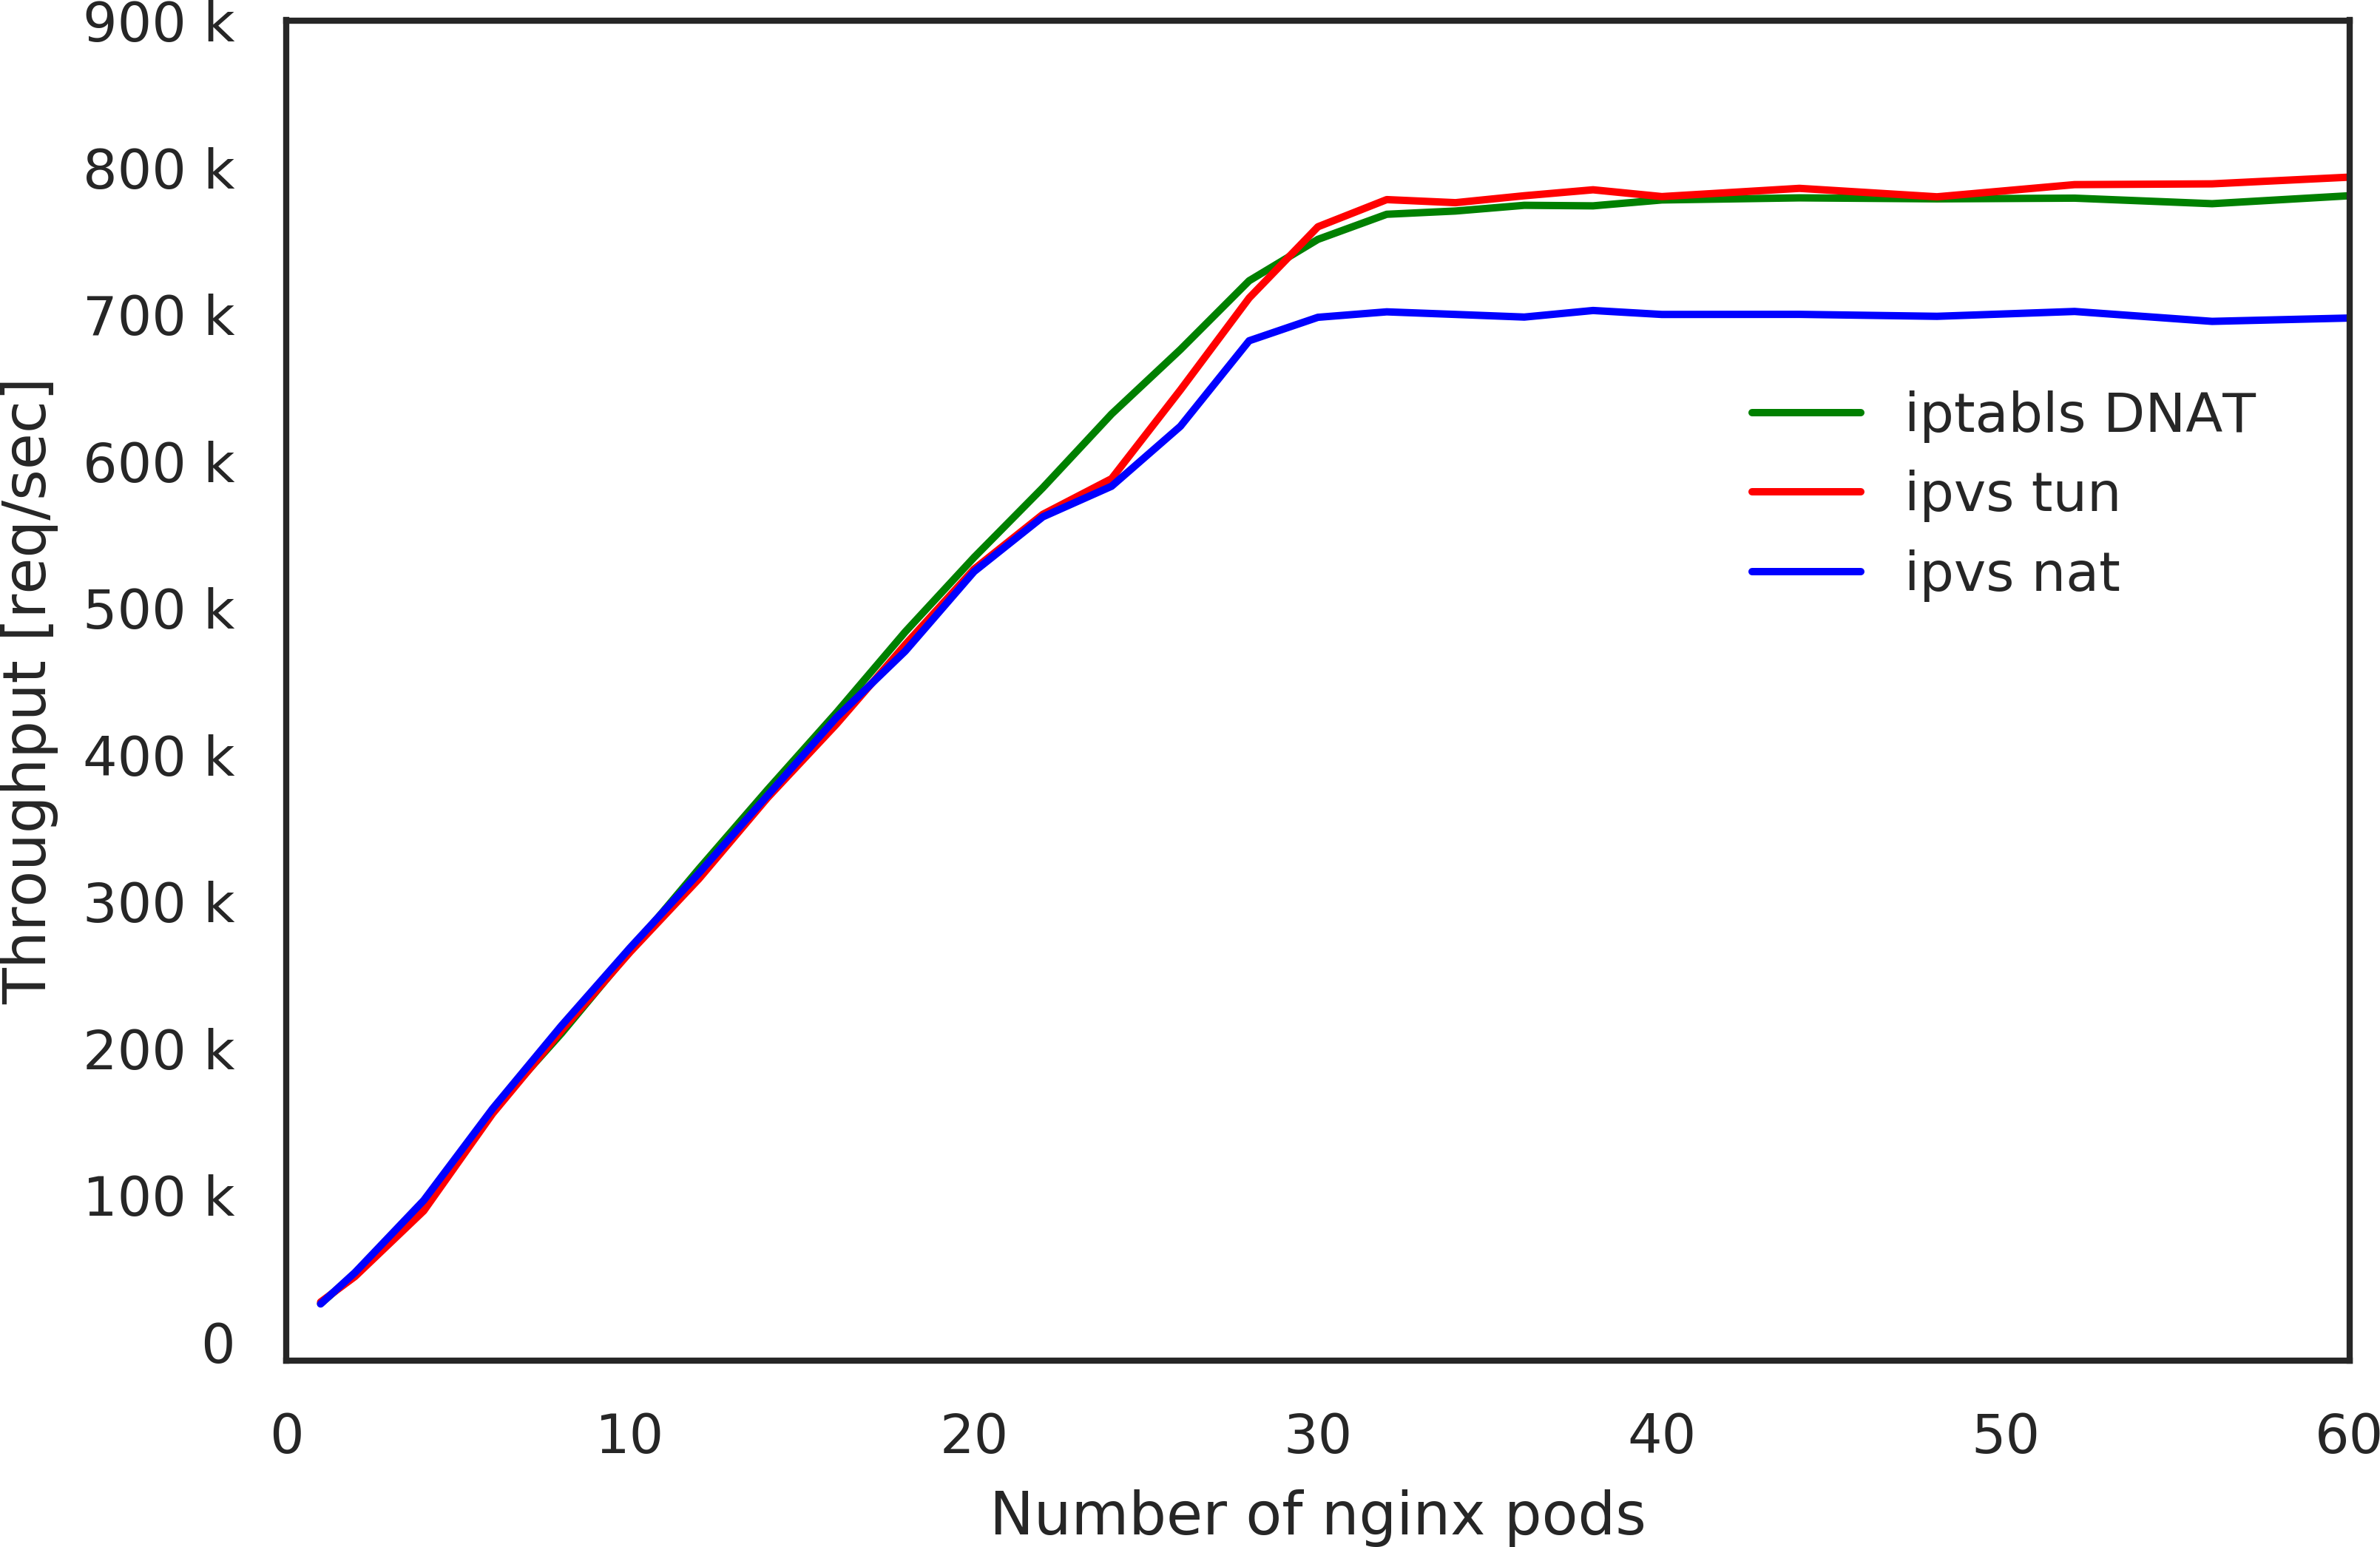
\includegraphics[width=0.8\columnwidth]{Figs/ipvs_node_l3dsr_10g}
  \par\bigskip
  \centering
  \begin{minipage}{0.9\columnwidth}
    \caption[Throughput of load balancers in node namespace]{
      Throughput of load balancers in node namespace.
      The performance levels of the ipvs and ipvs-tun are greatly improved those in \ref{fig:ipvs_l3dsr_10g} by placing them in node net namespace.
    }
    \label{fig:ipvs_node_l3dsr_10g}
  \end{minipage}
\end{figure}

Figure~\ref{fig:cpu_usage_10g_node_ns} shows CPU usages of each of the load balancers.
While the CPU usage of the ipvs-tun becomes less than that of iptables DNAT, the CPU usage of the ipvs is still larger than that of iptables DNAT.
The author suspects that the ipvs program itself is less efficient than iptables DNAT.

\begin{figure}[h]
  \centering
  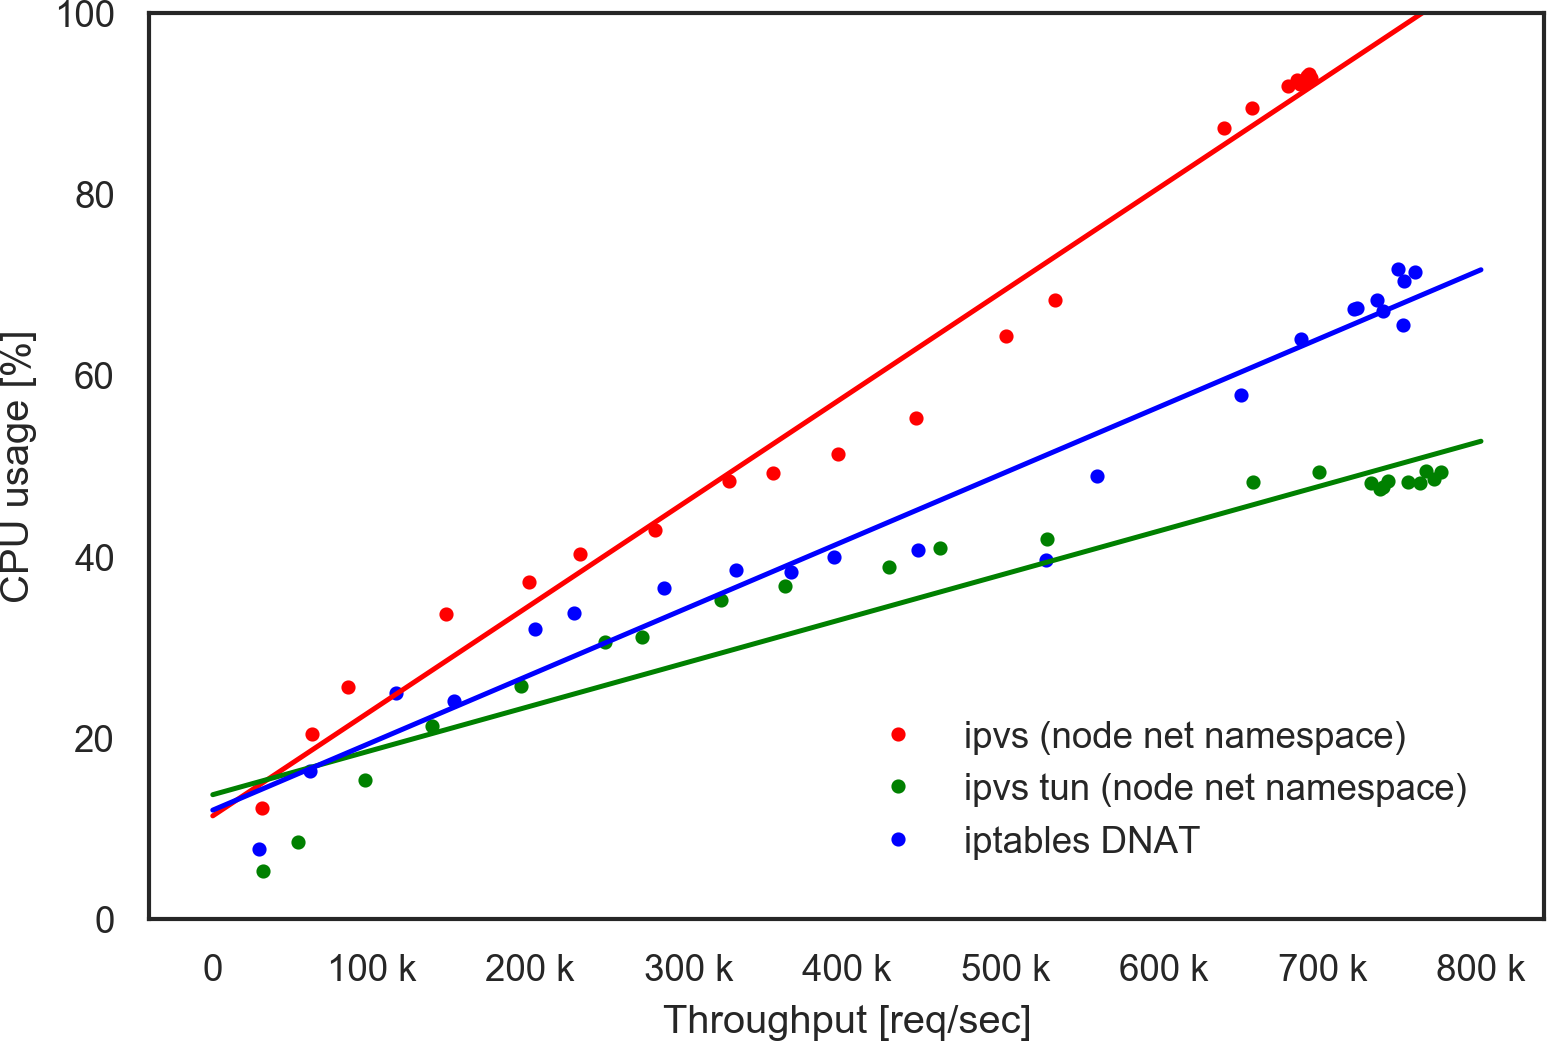
\includegraphics[width=0.8\columnwidth]{Figs/cpu_usage_10g_node_ns}
  \par\bigskip
  \centering
  \begin{minipage}{0.9\columnwidth}
    \caption[CPU usage of load balancers on nodes]{
      CPU usage of load balancers on nodes.
      The iptables DNAT rules on the node act as internal load balancer for Kubernetes.
      The ipvs and ipvs-tun are placed in node netnamespace for comparison. 
      The ipvs-tun consumes the smallest amount of the CPU resource.
    }
    \label{fig:cpu_usage_10g_node_ns}
  \end{minipage}
\end{figure}

The author summarizes this section as follows;
The performance levels of ipvs and ipvs-tun are inferior to that of iptables DNAT.
By placing ipvs and ipvs-tun in node net namespaces, their maximum throughputs and efficiencies have greatly improved.
However, the performance level and efficiency of the iptables load balancer are still better than those of ipvs.
Therefore, lesser performance levels for ipvs are both due to that fact that the container network causes overhead and that ipvs is less efficient than iptables DNAT.

\FloatBarrier

\section{Discussions of performance limitation}

The author has compared the performance of proposed load balancers in 10Gbps.
The proposed load balancer may not be the most efficient one, and there are rooms for improvement in container setup and the load balancer program itself.
However, it can be still usefull because of the lateral scalability.
And it is also essencial to understand how much of the traffic the load balancers need to accomodate.
In this section the author discusses that.

Table~\ref{tab:performance_summary} summarizes the maximum throughputs of the different load balancers obtained in all of the experiments.
Depending on the experimental conditions different part of the experimental setup becomes the performance bottleneck.
Since the performance bottlenecks of the 1Gbps experiments are due to network bandwidth of either load balancer or benchmark client, we can easily estimate the possible bottleneck due to bandwidth in a faster network.
Because the benchmark client exists at the location where normally the upstream router exists, the performance bottleneck at the benchmark client corresponds to the maximum throughput that load balancers are required to accommodate.

Since the bottleneck at the benchmark client is about 292K [req/sec], the load balancers are required to accommodate at most the throughput of 292K [req/sec] in the 1Gbps network.
This can be easily achieved by single ipvs-tun or two of ipvs load balancers with ECMP redundancy.

In the case of 10Gbps network, the performance bottleneck at the benchmark client is estimated to be 2.9M [req/sec], and hence the load balancers are required to accommodate at most throughput of 2.9M [req/sec].
This is still easily achievable by using four ipvs-tun or nine of ipvs load balancers with ECMP redundancy.

In the case of 100Gbps network, where the load balancers are required to accommodate up to throughput of 29M [req/sec], the inefficiency of the software load balancer in a container can become a real problem.
In the next section, the author tries to improve the efficiency of a load balancer, by implementing novel XDP load balancer.

\begin{table}[h]

  \begin{subtable}{1\textwidth}
    \centering
    \begin{tabular}{|l|l|c|l|}
      \hline
      \multicolumn{1}{|c|}{Type} & \multicolumn{1}{c|}{namespace} &
      \begin{tabular}{c} Throughput \\ {[}req/sec{]} \end{tabular} & \multicolumn{1}{c|}{Bottleneck} \\ \hline
      iptables DNAT & node      & 193.2K &
      \begin{tabular}{l} Bandwidth filled with request \\ + response @ load balancer \end{tabular} \\ \hline
      ipvs          & container & 196.7K &
      \begin{tabular}{l} Bandwidth filled with request \\ + response @ load balancer \end{tabular} \\ \hline
      ipvs-tun      & container & 292.7K &
      \begin{tabular}{l} Bandwidth filled with response \\ @ benchmark client  \end{tabular} \\ \hline
    \end{tabular}
    \caption{1Gbps experiment}
  \end{subtable}

  \par\bigskip

  \begin{subtable}{1\textwidth}
    \centering
    \begin{tabular}{|l|l|c|l|}
      \hline
      \multicolumn{1}{|c|}{Type} & \multicolumn{1}{c|}{namespace} &
      \begin{tabular}{c} Throughput \\ {[}req/sec{]} \end{tabular} & \multicolumn{1}{c|}{Bottleneck} \\ \hline
      iptables DNAT & node      & 777.6K & \begin{tabular}{l} CPU\(\sim\)100\% @ benchmark client\end{tabular} \\ \hline
      ipvs          & container & 334.8K & \begin{tabular}{l} CPU\(\sim\)100\% @ load balancer node\end{tabular} \\ \hline
        ipvs-tun      & container & 731.0K & \begin{tabular}{l} CPU\(\sim\)100\% @ load balancer node\end{tabular} \\ \hline
          ipvs          & node      & 699.6K & \begin{tabular}{l} CPU\(\sim\)100\% @ load balancer node\end{tabular} \\ \hline
      ipvs-tun      & node      & 779.9K & \begin{tabular}{l} CPU\(\sim\)100\% @ benchmark client\end{tabular} \\ \hline
   \end{tabular}
      \caption{10Gbps experiment}
  \end{subtable}

  \par\bigskip
  \centering
  \begin{minipage}{0.9\columnwidth}
    \caption[Summary of the maximum throughputs]{
      Summary of the maximum throughputs.
    }
    \label{tab:performance_summary}
  \end{minipage}
\end{table}

\section{XDP load balancer}

The eXpress Data Path(XDP) is Linux kernel technology recently developed, where the tools and functionality to incept and process the packets in the earlist phase as possible are provided.
By utilizing XDP, one can hook a byte-compiled code developed in subset of the C programing language, to a place before the socket buffer is assigned, thereby speeding up network manupulation, including block against DDOS atack, simple packet forwarding and load balancing.
The one of the benefit of the XDP compared to DPDK is that in the case XDP, the packtes that do not match the rule for processing are then passd to normal Linux network stack.
Therefore there is no need for preparing dedicated NIC for fast and efficient network processing.
The author implemented the XDP load balacer and carried out throughput measurement.

\subsubsection{Implementation}

\subsubsection{Benchmark setup}

\subsubsection{Throughput results }



\begin{figure}[h]
  \centering
  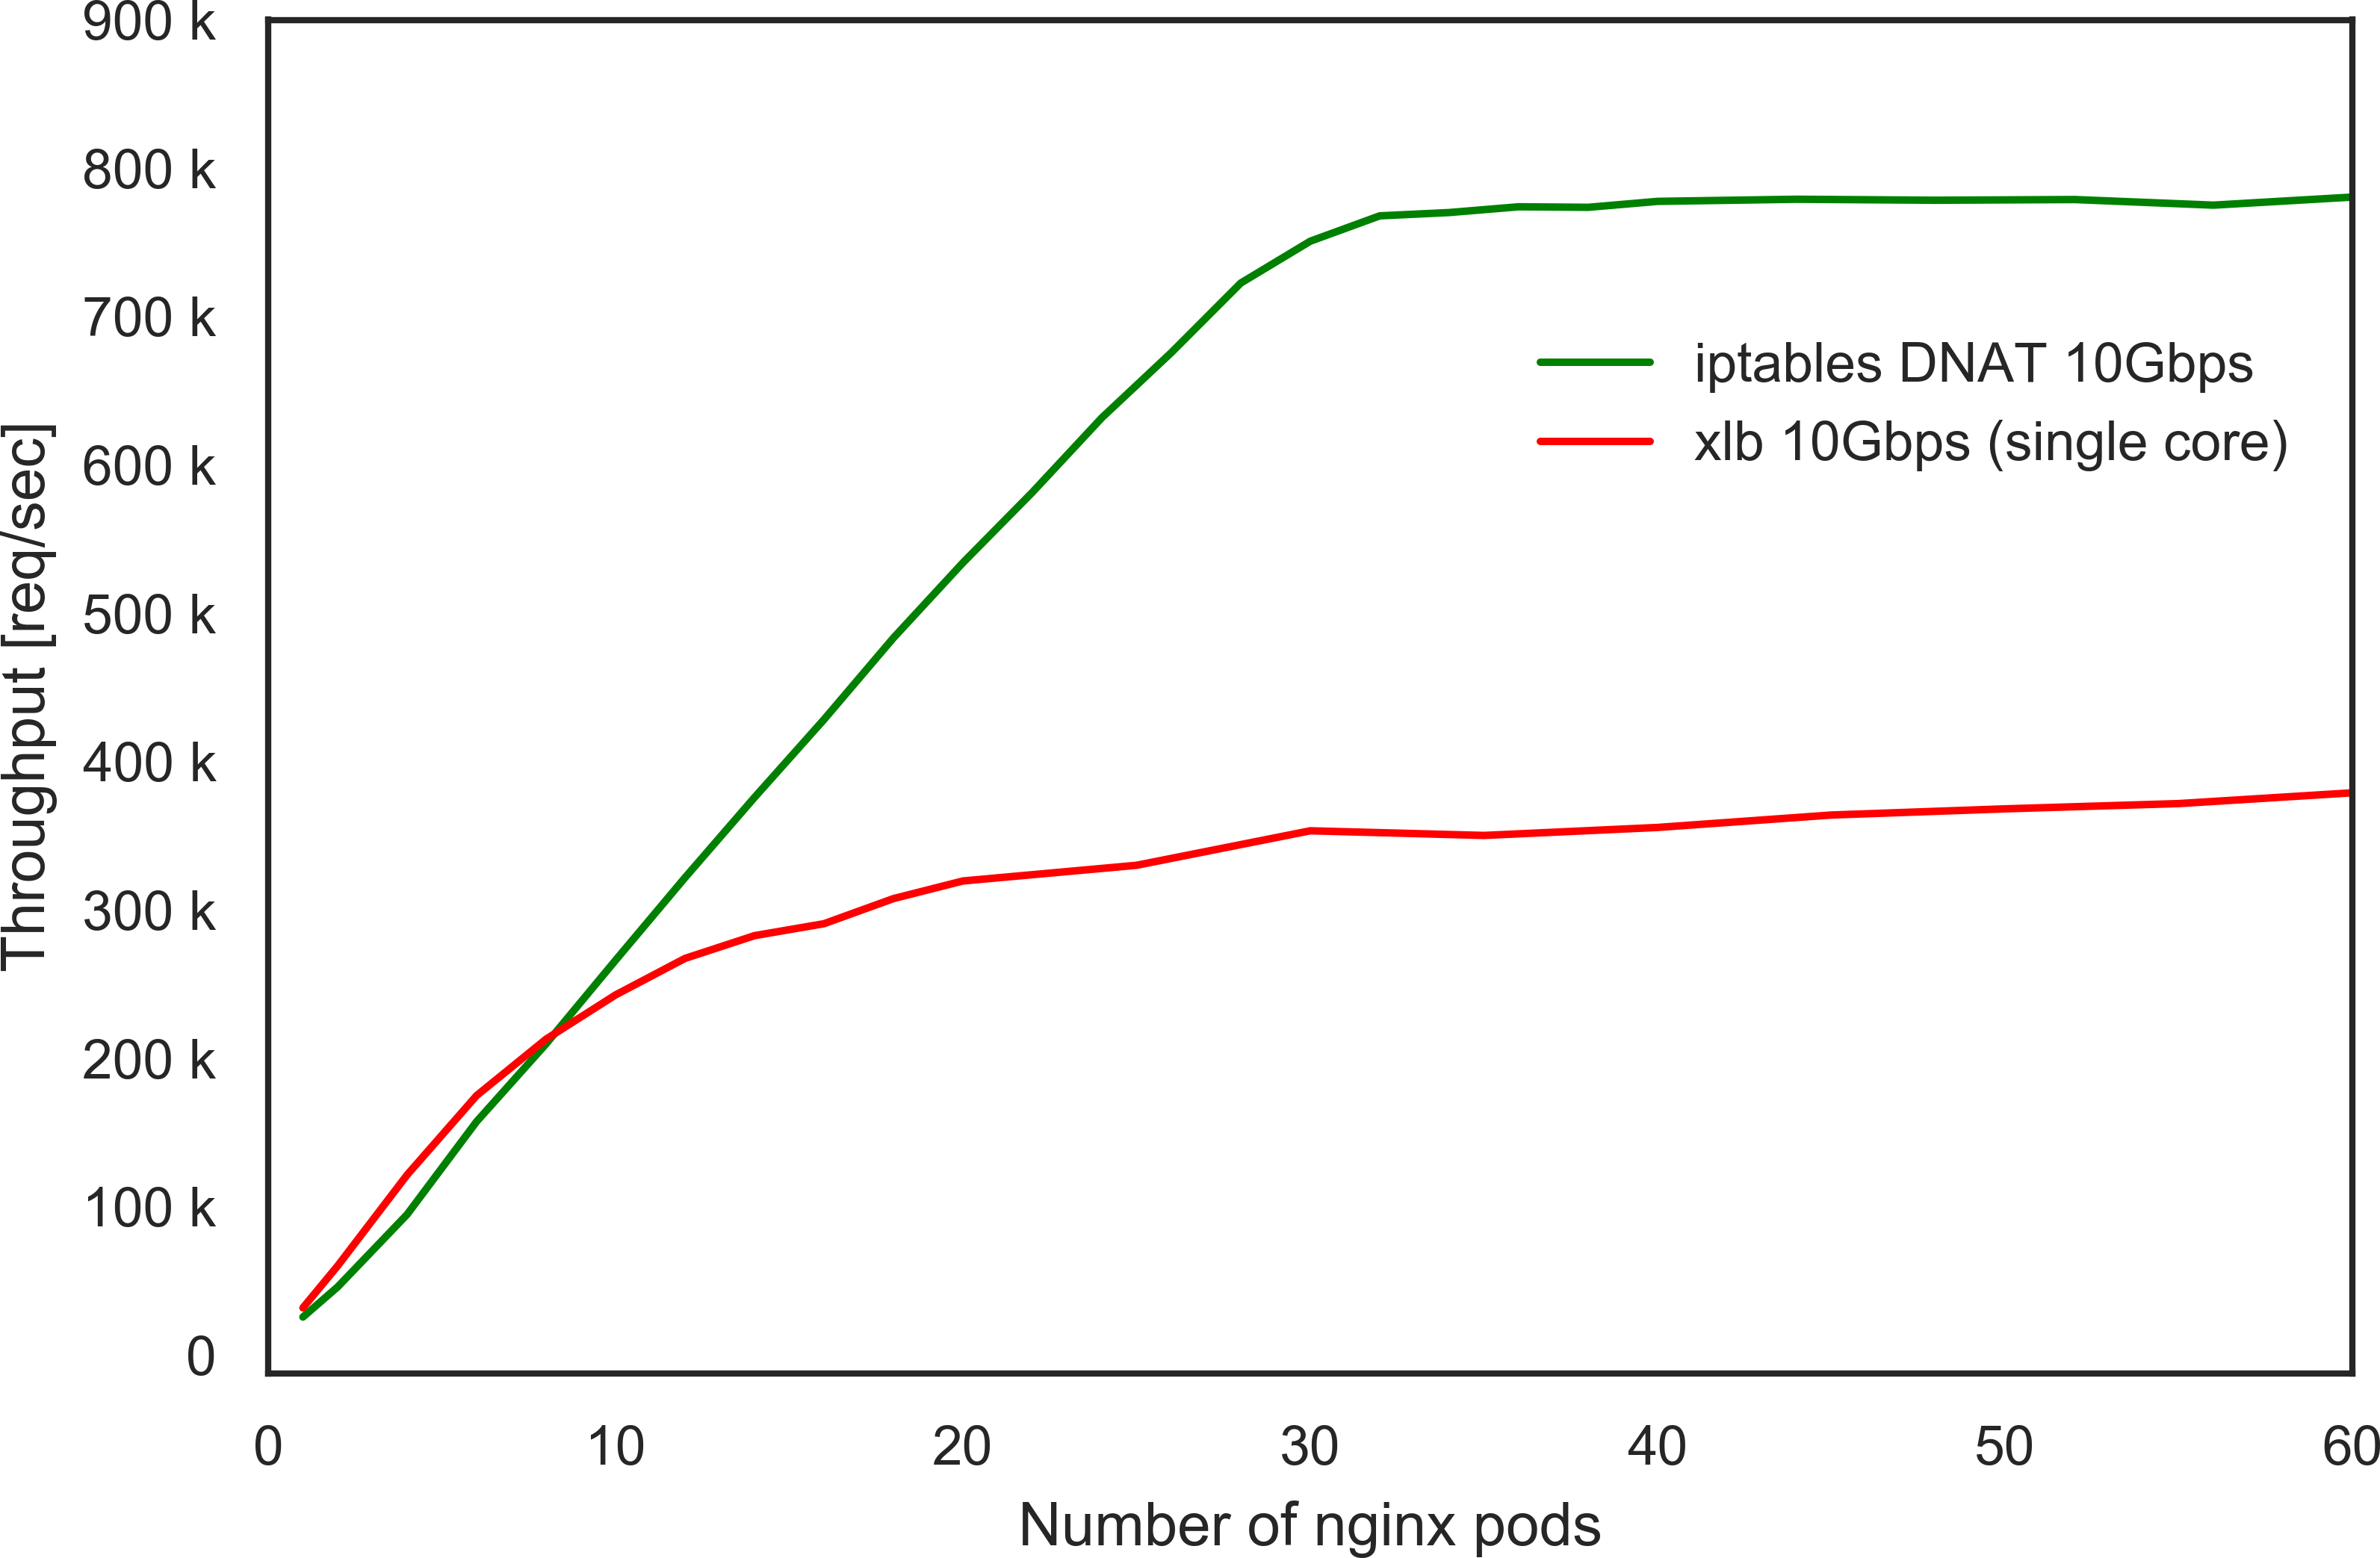
\includegraphics[width=0.8\columnwidth]{Figs/xlb_iptables_dnat_10g}
  \par\bigskip
  \centering
  \begin{minipage}{0.9\columnwidth}
    \caption[Throughput of xlb load balancer]{
      Throughput of xlb load balancer.
      The xlb load balancer is placed in node netnamespace.
      The setting \enquote{(RSS,RPS)=(off,off)}, i.e., single core packet processing is used for the xlb result.
      The setting \enquote{(RSS,RPS)=(on,off)}, i.e., eight core packet processing is used for the iptables DNAT result.
      Although using only a single core, the performance level of the xlb load balancer is close to half of the iptables DNAT's.
    }
    \label{fig:xlb_iptables_dnat_10g}
  \end{minipage}
\end{figure}


\begin{figure}[h]
  \centering
  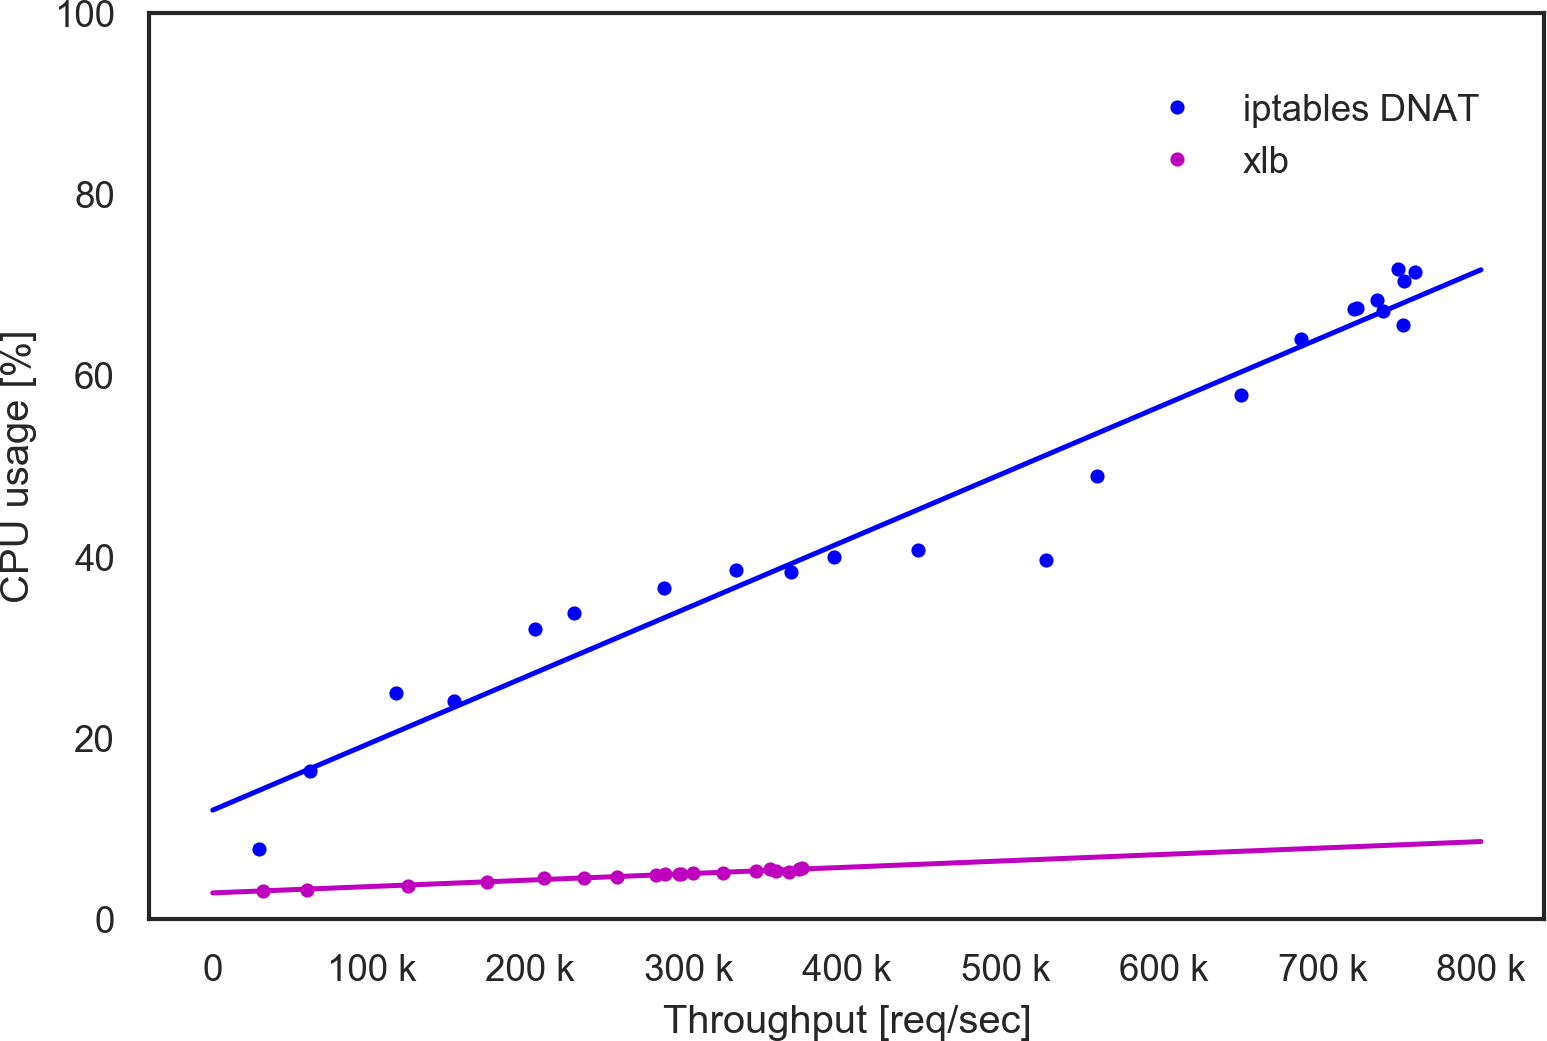
\includegraphics[width=0.8\columnwidth]{Figs/cpu_usage_10g_xlb}
  \par\bigskip
  \centering
  \begin{minipage}{0.9\columnwidth}
    \caption[CPU usage of xlb load balancer]{
      CPU usage of xlb load balancer.
      The xlb uses much less CPU resource than iptables DNAT.
    }
    \label{fig:cpu_usage_10g_xlb}
  \end{minipage}
\end{figure}

\FloatBarrier

\section{Summary}

In this chapter, the author carried out throughput measurements of ipvs-nat, ipvs-tun, and iptables DNAT in 10Gbps environment.
From the results the general characteristics of a load balancer are observesd.
The throughput increases linearly to a certain level as the number of nginx container increases, and then eventually saturates.
The performance levels for of the load balancers are improved by using 10Gbps network.
However, the throughputs of ipvs-nat and ipvs-tun are smaller than that of iptables DNAT.

Then the author improved the performance levels by setting up ipvs-nat and ipvs-tun load balancers in the node net namespace to remove overhead of the container network.
The throughput of the ipvs-tun became almost identical to that of iptables DNAT, and the throughput of the ipvs-nat also improved to the level close to that of the iptables DNAT.

%% The authot also presented the novel software load balancer using eXpress Data Plane(XDP) technology, as an alternative to ipvs software load balancers.
[Filled in later]
\mytodo[inline]{Write summary about XDP}



Load balancer in containers under performed and consumed more CPU resources than iptables DNAT on a node.
Container network that utilize bridge+veth maybe inefficient.
Better network set up for container is needed.

Maximum throughputs of ipvs-tun on a node and iptables DNAT are equivalent in the experiment, which is because the benchmark client can not measure throughput more than 800K [req/sec].
However the ipvs-tun consumed less CPU resouces than iptables DNAT.
Performance level of ipvs on the node is lower than of iptables DNAT.
The ipvs consumed more CPU resources than iptables DNAT.
Better software load balancers are needed.

The xlb load balancer has better per core throughput than iptables DNAT.
The xlb load balancer much less CPU resources than iptables DNAT.
The author plan to improve the perfomance levels of the xlb load balancer by enabling multicore packet processing. 


Band width limitations of 10G are 1.9M req/sec and 2.7M req/sec for ipvs and ipvs-tun, respectively.
Neither ipvs and iptables DNAT does not have that levels of performance. 

